% This template was initially provided by Dulip Withanage.
% Modifications for the database systems research group
% were made by Conny Junghans,  Jannik Strtgen and Michael Gertz

\documentclass[
     12pt,         % font size
     a4paper,      % paper format
     BCOR=10mm,version=first,     % binding correction
     DIV=14,version=first,        % stripe size for margin calculation
%     liststotoc,   % table listing in toc
%     bibtotoc,     % bibliography in toc
%     idxtotoc,     % index in toc
%     parskip       % paragraph skip instad of paragraph indent
     ]{scrreprt}

%%%%%%%%%%%%%%%%%%%%%%%%%%%%%%%%%%%%%%%%%%%%%%%%%%%%%%%%%%%%

% PACKAGES:

% Use German :
\usepackage[english]{babel}
% Input and font encoding
\usepackage[utf8]{inputenc}
\usepackage[T1]{fontenc}
% Index-generation
\usepackage{makeidx}
% Einbinden von URLs:
\usepackage{url}
% Special \LaTex symbols (e.g. \BibTeX):
%\usepackage{doc}
% Include Graphic-files:
\usepackage{graphicx}
% Include doc++ generated tex-files:
%\usepackage{docxx}
% Include PDF links
%\usepackage[pdftex, bookmarks=true]{hyperref}
\usepackage{csquotes}
\usepackage{color, colortbl, tabularx, ragged2e}
\definecolor{LightCyan}{rgb}{0.88,1,1}
\newcolumntype{C}{>{\raggedright\arraybackslash}X} % centered "X" column
% Fuer anderthalbzeiligen Textsatz
\usepackage{setspace}

% hyperrefs in the documents
\usepackage[bookmarks=true,colorlinks,pdfpagelabels,pdfstartview = FitH,bookmarksopen = true,bookmarksnumbered = true,linkcolor = black,plainpages = false,hypertexnames = false,citecolor = black,urlcolor=black]{hyperref} 
%\usepackage{hyperref}


%%%%%%%%%%%%%%%%%%%%%%%%%%%%%%%%%%%%%%%%%%%%%%%%%%%%%%%%%%%%

% OTHER SETTINGS:

% Pagestyle:
\pagestyle{headings}

% Choose language
\newcommand{\setlang}[1]{\selectlanguage{#1}\nonfrenchspacing}

\usepackage{biblatex}
\addbibresource{references.bib}

\begin{document}

% TITLE:
\pagenumbering{roman}
\begin{titlepage}
     \vspace*{1cm}
     \begin{center}
          \vspace*{3cm}
          \textbf
          {
               \Large University of Heidelberg\\
               \smallskip
               \Large Institute for Computer Science\\
               \smallskip
               \Large Working group database systems\\
               \smallskip
          }

          \vspace{3cm}

          \textbf{\large Bachelor thesis}

          \vspace{0.5\baselineskip}
          {
               \huge
               \textbf{Integrating Identity Management Providers based on Online Zugangs Gesetz}
          }

     \end{center}

     \vfill
     {
          \large
          \begin{tabular}[l]{ll}
               Name:                 & Jonas Gann              \\
               Matriculation number: & 3367576                 \\
               Supervisor:           & Prof. Dr. Michael Gertz \\
               Date of submission:   & \today
          \end{tabular}
     }

\end{titlepage}

\onehalfspacing

\thispagestyle{empty}

\vspace*{100pt}
\noindent
I assure that I have written this bachelor thesis on my own and only used the specified sources and resources and that I followed the principles and recommendations "Responsibility in Science" of the University of Heidelberg.

\vspace*{50pt}
\noindent

\underline{\phantom{mmmmmmmmmmmmmmmmmmmm}}

\medskip
\noindent
Date of Submission: \today
\newpage

\chapter*{Zusammenfassung}

\newpage

\chapter*{Abstract}

\newpage

\tableofcontents
\cleardoublepage
\pagenumbering{arabic}

\chapter{Introduction}

\section{Context}
Since invention of the World Wide Web, the number of its users increased rapidly. Today, more than 90 percent of the German population use the internet \cite{Onlinestudie}. Enterprises and organizations, recognised this potential to provide their services to a large number of people as Service Providers (SP). A frequently used method of SPs is "online self-service" (OSS). Specialized software tools enable customers to use services through the internet without direct human interaction.

Many tools require identification of a user in case interactions or initiated business processes have to be associated with him. A system for management of identities of users therefore is part of numerous system architectures. Service Providers usually enable users to manage their partial identities using online self-service through so called User Profiles. Today, customers of SPs are associated with multiple partial identities and user profiles - one for each SP

The result is variety of problems in management of digital identities \cite{IdentityCrisis}. Here are some examples:
\begin{itemize}
    \item Multiple SPs collect, use and share parts of identities which leads to distributed and fragmented identities.
    \item As a result of the distributed identities, risk of data breaches increases.
    \item Managing multiple use profiles is very inconvenient for users.
    \item It is often unclear who stores which data and for what purpose.
    \item SPs have an incentive to collect and share more user data than they need.
\end{itemize}

An improved model for identity management is necessary. In recent years, multiple new models have been invented. One model called Social Login became popular. It enables customers to create User Profiles for SPs through existing User Profile of Social Networks like Facebook. This improves identity management by enabling SPs to rely on the external profile for unique identification, authorisation and personal attributes. Users can therefore manage identity related information through their Social Profile which is accessed by the SP.

This approach, however, still leaves the requirement of User Profiles for each SP because, depending on the provided service, additional attributes which are not part of the Social Profile, have to be manageable by the user. SPs also might require additional online self-service tools the social network does not provide.

The solution to this problem is an Identity Management Provider (IMP) which manages the whole online identity of a person and can replace the individual partial identities and User Profiles. The system itself is provided and hosted by a SP for consumption by other SPs. To replace existing User Profiles, the IMP can not only rely on systems for registration, authentication, authorisation and provisioning. Additional requirements of SPs like communication, data wallet and management of additional attributes have to be satisfied.

In order for an SP to use identities and services of an IMP, an integration into the system architecture of the SP has to take place. Due to the complex nature of system architectures and identity management, this is a difficult task.

A currently relevant example for usage of online self-service with particular interesting requirements for identities is the German "Online Access Law" (Online Zugangs Gesetz: OZG). It requires all administrative services of the German federal republic, each member state and commune to be digitally available through interoperable user profiles. The current plan is to make the profiles only available for usage in context of the OZG. From a user perspective, this would be yet another partial identity and user profile to manage.

\section{Objective}
Based on the prominent example of the OZG, the bachelor thesis will construct a message based integration architecture which enables system architectures of service providers with existing user profiles to make their services usable with an Identity Management Provider. In order to make the integration architecture suitable to real life requirements, the OZG is selected as an example due to its current relevance and high requirements regarding identity management. The integration architecture is however not only applicable in cases relevant for OZG but also for other Service Providers with similar requirements. As requirements of SPs are not guaranteed to be similar to those of the OZG, the integration architecture is built to be expendable.

The \textbf{integration architecture} for the OZG enables \textbf{IMP functionalities} to be usable for selected \textbf{OZG scenarios} by integrating a \textbf{connector} in the \textbf{system architecture} of a member state.

\begin{itemize}
    \item OZG scenarios are based on documented digitalization efforts of administrative services in the context of the OZG and are for example the application for an administrative service or the communication with a governmental institution.
    \item The system architecture is based on documentation about architecture plans of member states.
    \item The functionalities of the IMP are based on a requirements analysis of OZG scenarios and additional research.
    \item The connector is defined based on functionalities the integration architecture requires from the IMP.
    \item The integration architecture is the main scientific contribution of this bachelor thesis. It is based on messaging patterns in order to utilize a combination of established and tested messaging solutions. In order to save investments it also reuses as many system components as possible and modifies as few system components as necessary.
\end{itemize}

The integration architecture ...

\section{Structure of Work}
The "Fundamentals" chapter explains terminology and basic concepts.

In the following chapter called "Identity Management System" the thesis analyzes requirements for identity management through the perspective of the user and through the perspective of service providers for the OZG. It is presented, how an identity management provider could solve current identity management problems and which challenges for an integration exist.

The chapter "Integration Proposal" first documents a possible IMP system and connector, based on the requirement analysis of the previous chapter. It then presents the integration architecture with iteratively increasing requirements through textual description, multiple flow diagrams and messaging architectures.

A "Solution Evaluation" analyzes benefits and problems of the proposed solution.

The "Outlook" will conclude the thesis by presenting possibilities for advanced integration architectures.

\chapter{Background and Related Work}

\section{Terminology}

\paragraph{Service Provider}
Service providers (SP) are entities like enterprises or organisations which make services accessible over the internet.

\paragraph{Online Self-Service}
Online self-service (OSS) describes a method used by Service Providers to make their services available to the user. The method is characterized by being available over the internet, requiring no direct human interaction but instead enabling the user to access services in a self-reliant way. The user is usually supported by a variety of software solutions.

\paragraph{Self-Service Tools}
Self-service tools are software solutions for customers to enable a online self-service experience. Depending on the use case, the tools can be transactional or informing. Informing tools help users to retrieve relevant information, often replacing human customer support. Transactional tools help users to interact with services in a persistent way to for example save personal data or trigger business processes.

Information tools can be for example so called "WiKi" pages or search fields which assist the user in his process of finding information. Transactional tools can be for example online forms which assist the user in his process of triggering an order placement business process.

In contrast to information tools, transactional tools often require identification of users in order to associate them with changes they made to the system: If a user triggers the business process of ordering a product, the SP requires identification of the user.

\paragraph{Digital Identity}
The digital identity, for simplicity called identity in the thesis, is the sum of all digital personal information. Each piece of personal information is an attribute. Attributes can be identifiers which are able uniquely identify an entity. It is also possible to use an aggregation of attributes as identifier.

Identifiers which are commonly used by SPs are the phone number and E-Mail address. Attributes are for example nicknames, hobbies, interests or education. The full name of a person is often not sufficient unique identification, the aggregation of name, age and home address can therefore be used as identifier.

\paragraph{Partial Digital Identity}
A partial digital identity is a subset of an identity. Partial identities are commonly used by SPs to manage identity information which is relevant for them. 

\paragraph{Identity Management}
Identity management is the creation, utilization / reading , updating and deletion of identities or partial identities. The possible utilization of identities depends on the system for management of identities. It could be for example authorization for a service or communication through an inbox.

\paragraph{Identity Management System}
Identity management systems are solutions which enable SPs and customers to manage identities or partial identities.
They usually provide the following functionalities an properties:
\begin{itemize}
    \item 
\end{itemize}

\paragraph{User Profile}
User profiles are one method for identity management. They are characterized by each SP providing a separate identity management system which often consist of an identity provider (IdP) for storing identities, a customer relation management system (CRM) for accessing identities internally and a website with online self-service tools for providing access to customers.

\section{Identity Management Provisioning (IMP)}
Identity management provisioning (IMP) is a method for identity management which is characterized by an identity management provider hosting an identity management system for "non-partial" identities. The identity management system provides one-stop online self-service for users and manages the storage of identities. SPs are provided access to the identities of the identity management system.

The following are functionalities of an IMP system in addition to those of conventional identity management systems:

\paragraph{Attribute Management}
It is common for identity management systems to enable users to manage a predetermined set of attributes. IMP systems however do not just manage partial identities and therefore enable users to manage any possible attribute of their identity. Users therefore can add, remove and modify any attribute.

As often, attributes of a digital identity are defined by service providers, they are also able to create new attributes or delete and modify existing ones, if approved by the user. 

\paragraph{Online Self-Service}
Many attributes, especially those created by SPs, do not make sense to the user without context and my be heavily dependant on systems of a SP. Therefore, the IMP provides solutions for online self-service which supports the management of attributes.

\paragraph{Integration}
Service providers which use IMP systems as solution for identity management require access to its services and have to make their existing systems work with them. The IMP solution therefore provides interfaces which enable the SP to access services. As it is in the best interest of the IMP solution to integrate SPs, advanced integration methods reducing the integration effort for SPs can be provided. 

\section{Online Access Law (OZG)}
In 2017 the German government passed the law for improvement of online access to administrative services (Online Zugangs Gesetz: OZG) which requires federal republic and member states to execute the following regulations until 2022 \cite{BMI:OZG_Wortlaut}:
\begin{enumerate}
    \item \textbf{Digital availability of administrative services} \\
    An administrative service is the electronic processing of administrative procedures which are available from outside the governmental institution.  As it is not clear which administrative services exactly are meant by the definition of the OZG, the BMI created a catalogue \cite{BMI:Verwaltungsleistungen}. The OZG requires these services to be digitally available. As a guideline to what is considered sufficient availability, the BMI defined a maturity model \cite{BMI:Digitale_Services}.
    \item \textbf{Digital access to administrative services through administration portals of a portal network} \\
    Federal republic, each member state and each commune must provide an administration portal. Portals of communes must be linked to the portal of the corresponding member state. Portals of federal republic and member states must be connected through a portal network. \cite{BMI:Portalverbund} Each portal must provide a "seek and find" feature, which enables users to find all administrative services provided by any administration portal \cite{Cotar:Drucksache_19/19089}. 
    \item \textbf{Interoperable user profiles for accessing administrative services} \\
    Federal republic and member states must provide user profiles which can be used to identify the corresponding person while requesting access to administrative services, to save personal information according to the once-only principle, to receive and send messages via a digital mailbox and to pay for services \cite{Cotar:Drucksache_19/19089}. The user profiles must be interoperable for every administration portal of the portal network.
\end{enumerate}

Execution of the OZG can be separated into two projects:

\paragraph{Digitalization}
Digitalization of administrative services focuses on accessibility towards users but not modernization of its internal execution by administrative institutions. The goal of digitalization in this case is, to make administrative services available towards a user in a digitized way:

A digitized administrative service can be accessed by a user through a website. The website is hosted either by the federal republic or a member state and is called "Administration Portal". Access is usually provided through an application form. The administrative service can be managed through a user profile which is provided by the federal republic or the member state. Management of an administrative service usually includes starting the service by sending in a form, communicating with responsible institutions through the inbox of the profile and receiving a result. The user profile can also enable users to upload documents to a data wallet and to save personal information for automatically filling in forms.

Digitalization of an administrative service is the modification of the underlying processes to incorporate the usage of the described features of the user profile and administration portal. In total, the BMI lists 575 relevant services, some of them provided by the federal republic, some by the member states and yet other by the communes \cite{BMI:Onlinezugangsgesetz}.

\paragraph{Networking}
The networking focuses on connecting governmental systems to make all digitized administrative services available for every user. This includes most importantly the connection of administration portals to a portal network through an online gateway and the interoperability of user profiles.

In order to save investments a method called "one for all" is used when hosting administrative services. One member state or the federal republic provide access to a service on their administration portal and distribute the requests to the responsible institutions "under the hood". As administration portals are connected through an "online gateway", each portal contains a search feature, which enables users to find all administrative services through any portal. Interoperable user profiles enable usage of each profile for management of administrative services on all portals.

\subsection{Basic Use Case}
The BMI lists a total of almost 600 administrative services, each being described by a different process \cite{BMI:Informatiosplattform}. Each process consists of multiple sub-processes. When comparing the processes, one can see, that some sub-processes occur very often and in similar arrangements. Those arrangements can be called the basic use case of OZG services.

The basic use case describes the submission of an application for an administrative service and consists of the following arrangement of sub-processes \cite{NRW:Umsetzung}:

\paragraph{1. Selection of Administrative Service}
The user visits any administration portal of the portal network and types a search term in the corresponding search field. The user is then presented with a list of search results consisting of administrative services. If the user selects a search result, he is forwarded to the correct page inside the domain of the administration portal which hosts the selected service. This page provides information about the administration service along with instructions on how to access the form for application. The interactive form, usually provided by a form-server, can be for example included in the page through a web-component.

\paragraph{2. Login to User Profile}
Independent of the member state the user created the interoperable user profile for, he can use it in the current administration portal. The user has to finish authentication steps, which can consist for example of a username and password. Depending on the authentication method, a trust level of the current session is determined. With approval from the user, personal information from his profile is provided towards the form-server.

\paragraph{3. Filling in Application}
Personal information from the user profile is used by the form-server to fill as many fields of the form as possible. The form with prefilled information is then presented to the user. The interactive form can then be modified by the user. Depending on the form-server, additional functionalities like conditions between fields or sanity checking can be provided.

\paragraph{4. Uploading Attachments}
The user can upload documents to his user profile and reference them in the form.

\paragraph{5. Submission of Application}
The user again authenticates for his user profile and authorises the form-server to submit the application. The form-server saves the application until he is notified to delete it. The form-server submits the application to the administration portal which hosts the administrative service.

\paragraph{6. Reception of Application by Administration Portal}
The administration portal receives the application from a form-server and usually just forwards it to the data-exchange platform and notifies the form-server that the he can delete the application.

\paragraph{7. Submission of Application to Data-Exchange Platform}
The data-exchange platform distributes the application to the correct administrative institution responsible for processing it.

\paragraph{8. Sending of Acknowledgment}
The data-exchange platform notifies the user through the inbox functionality of the user profile if the application was submitted successfully.

\subsection{System Architecture}
This subsection describes the system architecture of a member state relevant for the execution the basic use case of the OZG based on the system architecture of Nordrhein-Westfalen. Systems, which are responsible for coordination of OZG execution between member states and the federal republic are not the focus.

\subsubsection{System Components}
The system architecture consists of the following system components. Each component consists of a list of services it provides either to the user or to other components. Components are defined based on strongly connected categories of services \cite{NRW:Umsetzung}:

\paragraph{Administration Portal}
The administration portal provides the user with a web-interface and implements user flows of digitized administrative processes by interacting with other system components. The main services are \cite{NRW:Umsetzung}:

\begin{itemize}
    \item \textbf{Search and find a form}
    
    Due to the distributed responsibility for provisioning administrative services through for example the "one for all" method, it is not clear to the user, which member state provides which administrative service on his portal. Therefore, each administration portal provides a "Search and Find" functionality, which enables the user to find the correct administration portal and page, where the service is provided. In order for the administration portals to provide the "Search and Find" feature, an "Online Gateway" makes information about the location of administrative services accessible through a central data storage \cite{Capgemini:OnlineGateway}.
    
    \item \textbf{Selection of administrative service}
    
    In combination with the "Search and Find" feature, the user can select an entry of the search result and is forwarded to the corresponding web-page. Depending on the administrative service, the web-page can be hosted on the current or a different portal. It shows information about the selected service like a service description, requirements and possible outcomes and enables the user to open the corresponding form hosted by a form-server.
    
    \item \textbf{Opening a form through a form-server}
    
    The web-page of an administration portal describing the administrative service can integrate a form-server in multiple ways. The maybe easiest way is to add an URL which forwards the user to a web-page provided by the form-server. More advanced integration methods are possible where the form is rendered inside the web-page of the portal.
    
    \item \textbf{Request of personal information from user profile}
    
    Each member state and the federal republic provide interoperable user profiles. The administration portal is able to access the services of every user profile, which includes retrieval of personal information stored in the user profile. This requires a user to be logged into his user profile with a sufficiently high trust level.
    
    \item \textbf{Transfer of personal data to the form-server}
    
    If the administration portal was able to retrieve personal information from a currently active user profile, it can, with approval of the user, transmit it to the form-server which provides the form corresponding to the selected administrative service.
    
    \item \textbf{Reception of applications from form-server}
    
    The administration portal can request the application data from the form-server after it was notified of its "submission".
    
    \item \textbf{Feedback to form-server}
    
    The administration portal notifies the form-server, that it no longer has to store a certain application.

    \item \textbf{Determination of receiving institution}
    
    Administrative services can be processed by a variety of administrative institutions, depending on the content of the application or the sender. It is the responsibility of the administration portal to determine which institution receives which application.
    
    \item \textbf{Transfer to data-exchange platform}
    
    The administration portal transfers the application to the data-exchange platform which is responsible for delivering it to the institution.
\end{itemize}

\paragraph{Form-Server}
The from-server provides digital forms associated to administrative services. They can be accessed by a user profile through online self-service and submitted as applications to administrative institutions. The main services are \cite{dNRW:Standardisierungskonzeptzur}

\begin{itemize}
    \item \textbf{Retrieval of a digital form}
    
    There exist many administrative services and depending on the member state or commune, the required layout of the application can be different. Therefore, a system called federal information management (Föderales Informationsmanagement: FIM) is used to standardize administrative services. FIM consists of three categories of building blocks.
    
    \textit{Service blocks} contain human readable descriptions about a administrative service.
    
    \textit{Data field blocks} contain the standardized description of data fields required for the application of administrative services.
    
    \textit{Process blocks} contain standardized descriptions about the process of an administrative service.

    Relevant for the form-server are data field blocks. A data field block can contain one element of five categories.
    
    \textit{Data fields} are the "smallest entity" of a data field block and describes one standardized piece of information. Depending on the type of information - if it is for example a checkbox or input field - additional metadata is included.
    
    \textit{Data field groups} consist of multiple data fields and other data field groups, relating to a category of information. A data field group can for example be "person" or "company".
    
    \textit{Rules} describe all kinds of logical conditions of and between data fields. This includes for example the automatic validation of the correctness of an entered value or the activation and deactivation of data fields depending on an entered value.
    
    \textit{Code lists} are lists of predefined values the user can select. This can for example be a list of all countries.
    
    \textit{Data field schemata} is the combination of entities from all previously described categories and describes the structure of a form.
    
    The building blocks are centrally managed by federal republic, member states and communes. This simplifies the creation of for example a new form by reusing existing data schema blocks and adding additional required data fields to a new data field schema.
    
    Each data field block can be uniquely identified through an ID. Therefore, if the form-server is provided with a FIM-ID, he can retrieve the corresponding data filed block from the central storage.
    
    \item \textbf{Initiation of application}
    
    The from-server can be requested to initiate an application using a certain form based on a FIM ID of a data field schemata. Along with the request, an identification and authorisation of a user profile has to be passed. Additional personal information of the user profile can be passed for automated filling in of the form.
    
    \item \textbf{Status update to portal}
    
    The form-server sends updates to the administration portal regarding the current status of the application. The possible status updates are listed in the interface section.

    \item \textbf{Automatic filling in of form}
    
    If the administration portal submitted personal data to the form-server, the form can automatically be filled in. This can be done because both the user profile and the form-server use the same data fields defined through FIM.
    
    \item \textbf{Presentation of form}
    
    The form can be integrated into the administration portal through for example an URL or Web-Component.
    
    \item \textbf{Application interruption}
    
    The application can be interrupted or aborted. Interruption may occur if the user stays inactive for a certain period of time while filling in the form. The user can also manually interrupt the editing process. If the application is interrupted, the form-server stores the unfinished application for a certain amount of time. The user can then access the application at a later time.
    
    If the user decides to cancel editing the form, the application is deleted from the from-server.
    
    Depending on the actions of the user, the status of the application changes accordingly and the administration portal is notified through a status update.
    
    \item \textbf{Storage of application}
    
    The form-server stores applications for a specified period of time if they were interrupted or submitted. In case of submission, the administration portal notifies the form server, if the application can be deleted.
    
    \item \textbf{Provisioning stored applications}
    
    The administration portal submits JWT to the form-server which corresponds to a user profile. Based on this information, the form-server searches all stored applications which belong to the user profile and sends back to the portal a list of URLs, through which the user can access them.
    
    \item \textbf{Deletion of stored application}

    If requested by the administration portal, the form-server can delete stored applications. This is usually the case after an application was submitted to the administration portal.

    \item \textbf{Manually filling in data fields}
    
    When the form is presented to the user, it can happen, that not all information could be automatically filled in. In this case, the form can be interactively filled in by the user.
    
    \item \textbf{Uploading documents}
    
    The user can add documents as attachments to an application. Uploaded documents are scanned for viruses.
    
    \item \textbf{Authentication of user profile}
    
    JSON web token from administration portal.

    \item \textbf{Submission of application}
    
    When the user submits the application by for example pressing a "submit" button, the form-server notifies the administration portal through a status update. The administration portal can then continue processing the application by requesting the application data from the form server. The portal does this by sending the form-server a FMS-ID it was sent by the form-server with the first status update. 
    
\end{itemize}

\paragraph{User Profile}
Each member state provides its own user profile for identity management. The main services are \cite{NRW:Umsetzung}:

\begin{itemize}
    \item \textbf{Identification and Authentification} \cite{dNRW:Anbindungsleitfaden}
    
    The user profile can be used for identification by transmitting personal information like name and address after successfully authentification. Authentification is the verification of an authentication. Users can authenticate for the user profile for example through a username / password combination.
    
    \item \textbf{Determination Trust Level} \cite{dNRW:Anbindungsleitfaden}
    
    The trust level of a logged in user profile is determined while registration and usage. The user can register and login to the user profile using a username / password combination or the German ID card. The trust level "High" is only granted, if the user registered using the German ID card \textbf{AND} logs in using the German ID card. All other combinations of registration and login result in a "normal" trust level.
    
    \item \textbf{Management Personal Information} \cite{dNRW:Anbindungsleitfaden} 
    
    Personal information of the user profile can be managed through the administration portal after successful authentication.
    
    \item \textbf{Provisioning Personal Information to Form-Server} \cite{dNRW:Anbindungsleitfaden} \cite{dNRW:Schnittstellen}
    
    If a user selects to open the form of an administrative service which is integrated in the administration portal, the portal asks the user for permission to transmit personal information to the form-server. If the user is logged in and accepts, the administration portal retrieves the necessary personal information from the user profile and forwards it to the form-server.
    
\end{itemize}

\paragraph{Institution}
Institutions are the entities which eventually process the incoming applications and provide the users with solutions. They receive a digital application through the data-exchange platform. Institution are provided a special website on the administration portal, where they can interact with the user of an application through for example messages, status updates or requests for additional documents. Those interactions are done manually by an employee through the user interface of the website but can, to some degree, be automated.

\paragraph{Data-Exchange Platform}
The data-exchange platform delivers applications from the administration portal to the correct administrative institution.

\paragraph{Data Wallet}

\paragraph{Inbox}

\subsubsection{Interfaces}
In order to implement the basic use case, the components have to interact with each. The following diagram visualizes, which components interact. Each interaction is described afterwards.

\begin{center}
    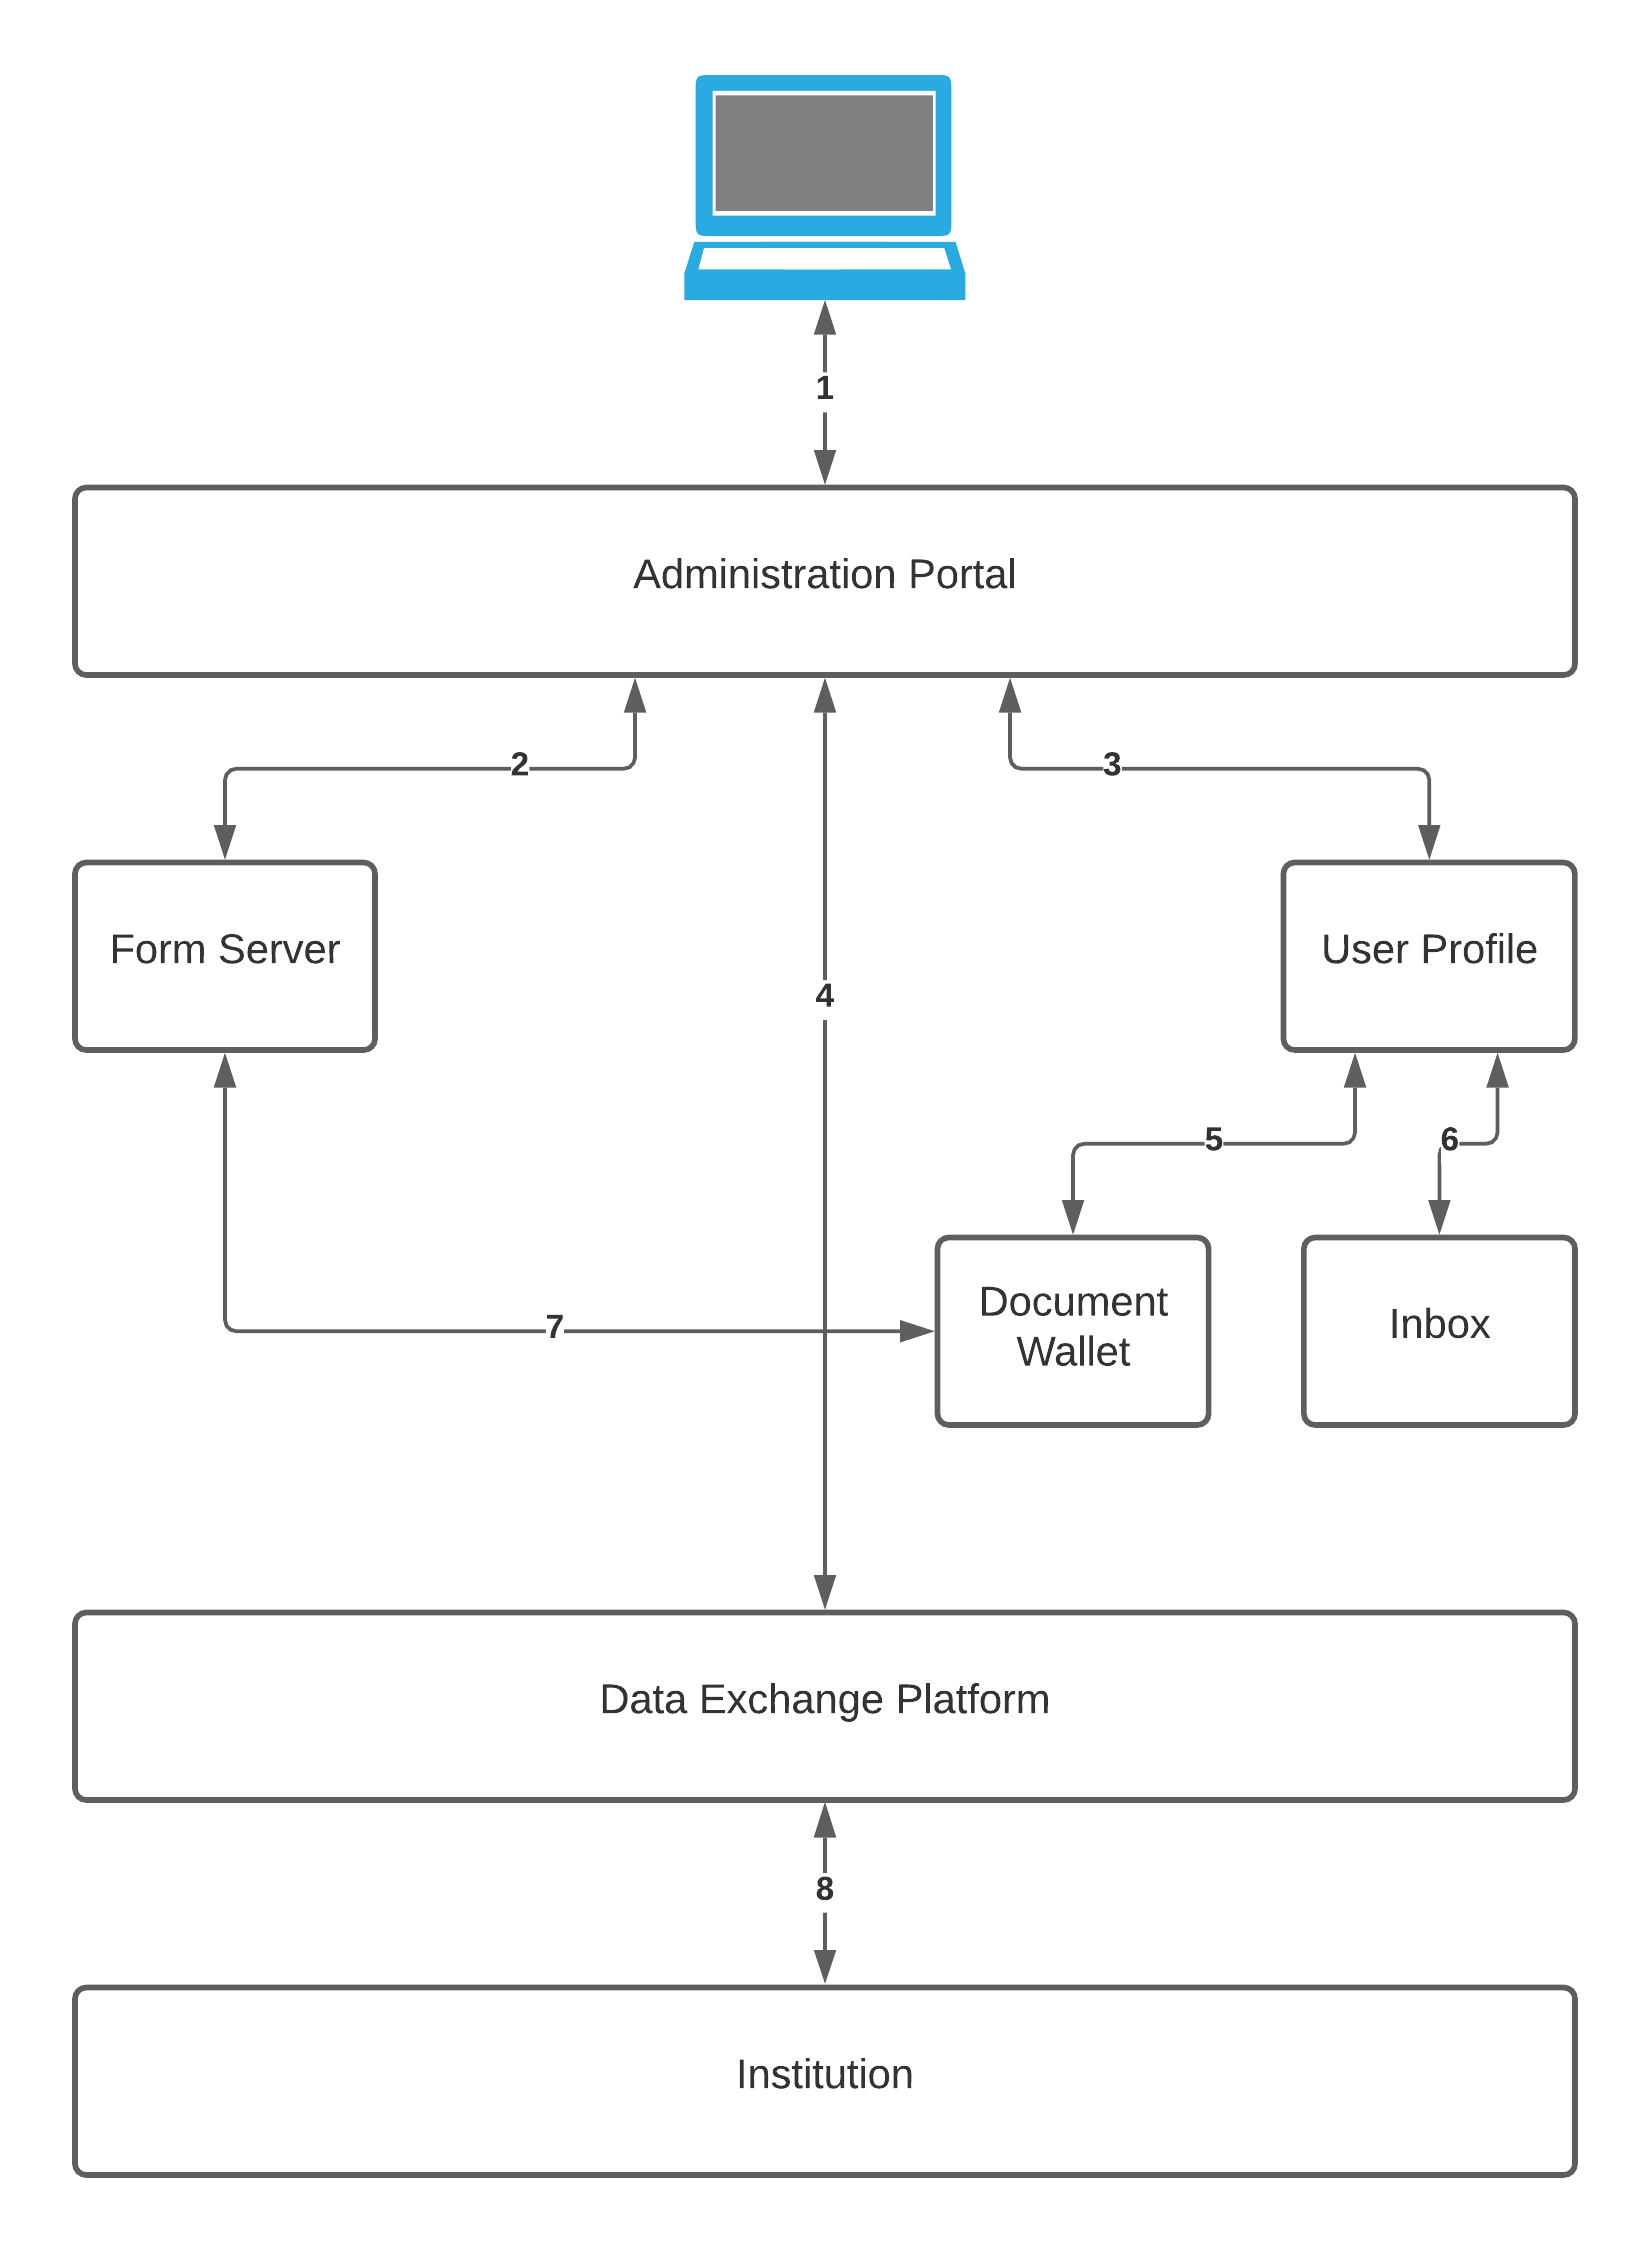
\includegraphics[width=8cm]{Interaction Diagram.png}
\end{center}

\begin{enumerate}
    \item The user interacts with the system architecture relevant for OZG only through the administration portal. The user is provided with a website as an interface with multiple online self-service functionalities.
    \item Administration portal and form-server interact through a REST API. The API provides the following interfaces:
    \begin{itemize}
        \item \textbf{Application initiation interface provided by form-server and used by administration portal}
        
        On the page of an administrative service on the administration portal, the user can press a button "to online application". Upon pressing the button, the portal interacts with the form server by transmitting data through an interface and receiving a response, see table \ref{table:interface_form_initialization}.
        
        \begin{table}[!h]
            \begin{tabularx}{\textwidth}{|l|C|l|}
            \hline
            Property & Description & Data Source \\
            \hline
            \rowcolor{LightCyan}
            \multicolumn{3}{|l|}{Input} \\
            \hline
            
            JSON Web Token & The portal received this JWT as a result of the login process with the user profile component. This token enables the form-server to verify the authentication of the user. & User Profile \\
            
            \hline
            
            User Profile ID & This ID is a unique identifier of a user profile and is used by the form server to associate the initiated application with a user profile. & User Profile \\
            
            \hline
            
            Personal Data & If the user approves, the administration portal submits personal data, the form-server can use to automatically fill in the form. & User Profile \\
            
            \hline
            
            FIM Schema ID & The administration portal stores a hard coded FIM-ID for every administration service. This FIM-ID corresponds to the correct data field schemata, the form-server can display & Hard Coded in Portal \\
            
            \hline
            \rowcolor{LightCyan}
            \multicolumn{3}{|l|}{Output} \\
            \hline
            
            Status & The form-server answers with the status of the initiated application. & From Server \\
            
            \hline
            
            FMS-ID & While initializing the application, the form-server creates an ID, which uniquely identifies the application. This FMS-ID is sent back to the portal so that it can request information about the application at a later time. & Form Server \\
            
            \hline
            \end{tabularx}
            \caption{Interface of the form-server for initialization of an application}
            \label{table:interface_form_initialization}
        \end{table}
        \item \textbf{Status updates from from-server to administration portal}
        
        The form-server notifies the administration portal of changes in the status of the application through an interface, see table \ref{table:interface_status}.
        
        \begin{table}[!h]
            \begin{tabularx}{\textwidth}{|l|C|l|}
            \hline
            Property & Description & Data Source \\
            \hline
            \rowcolor{LightCyan}
            \multicolumn{3}{|l|}{Input} \\
            \hline
            
            FMS-ID & The FMS-ID was created by the form-server during the initialisation of the application and sent to the administration portal. Each status update includes this ID in order for the portal to associate the update with an application. & Form Server \\
            
            \hline
            
            Status & The status provides information about interactions of the user or the form-server with the application. The possible states are:
            
            \begin{itemize}
                \item \textbf{null}: This application has this status right after initialisation.
                \item \textbf{submitted}: The application has this status after the user triggered the submit functionality of the form-server. Usually the form is now locked for further modification by the user.
                \item \textbf{filed}: The form-server submitted the application to the portal but did not yet receive a confirmation.
                \item \textbf{confirmed}: The form-server received a confirmation from the portal.
                \item \textbf{deleted}: The form-server deleted the application.
            \end{itemize}
            
            & Form Server \\
            \hline
            \end{tabularx}
            \caption{Interface of the administration portal for receiving status updates by the form-server}
            \label{table:interface_status}
        \end{table}
        
        \item \textbf{Submission of the application from the form-server to the administration portal}
        
        After the administration portal received the status update "submitted", it requests the form-server to transfer the application data through an interface, see table \ref{table:interface_application_data}.
        
        \begin{table}[!h]
            \begin{tabularx}{\textwidth}{|l|C|l|}
            \hline
            Property & Description & Data Source \\
            \hline
            \rowcolor{LightCyan}
            \multicolumn{3}{|l|}{Input} \\
            \hline
            
            FMS-ID & The FMS-ID was created by the form-server during the initialisation of the application and sent to the administration portal along with the status update of the submission. The administration portal sends this ID in order for the form-server to know which application data to transfer. & Form Server \\
            
            \hline
            \rowcolor{LightCyan}
            \multicolumn{3}{|l|}{Output} \\
            \hline
            
            FMS-ID & The FMS-ID is transmitted in order for the portal to associate the response with an application. & Form Server \\
            
            \hline
            
            JSON Web Token & The JWT which was initially sent from the portal to the form-server is now transmitted back again, in order for the portal to verify, that the form-server is authorized to submit an application for the user. & User Profile \\
            
            \hline
            
            User Profile ID & The user profile ID was initially transmitted to the form-server by the portal and is now transmitted back in order for the portal to associate the application with a user profile. & User Profile \\
            
            \hline
            
            XML File & The XML file contains the personal data retrieved through the form. & Form Server \\
            
            \hline
            \end{tabularx}
            \caption{Interface of the form-server for requesting application data by the administration portal.}
            \label{table:interface_application_data}
        \end{table}
    \end{itemize}
    
    \item The administration portal interacts with the user profile to provide online self-service for profile management and to identify the user and to request authentication and authorisation.
    
    \item The administration portal interacts with the data exchange platform to transfer an application which the data exchange platform submits to the correct institution.
    
    \item 
    
    \item
    
    \item
    
\end{enumerate}
    
\subsubsection{Data Objects}
The system architecture processes the following data objects which are associated to certain system components:

\subsection{Basic Use Case Sequence Diagram}

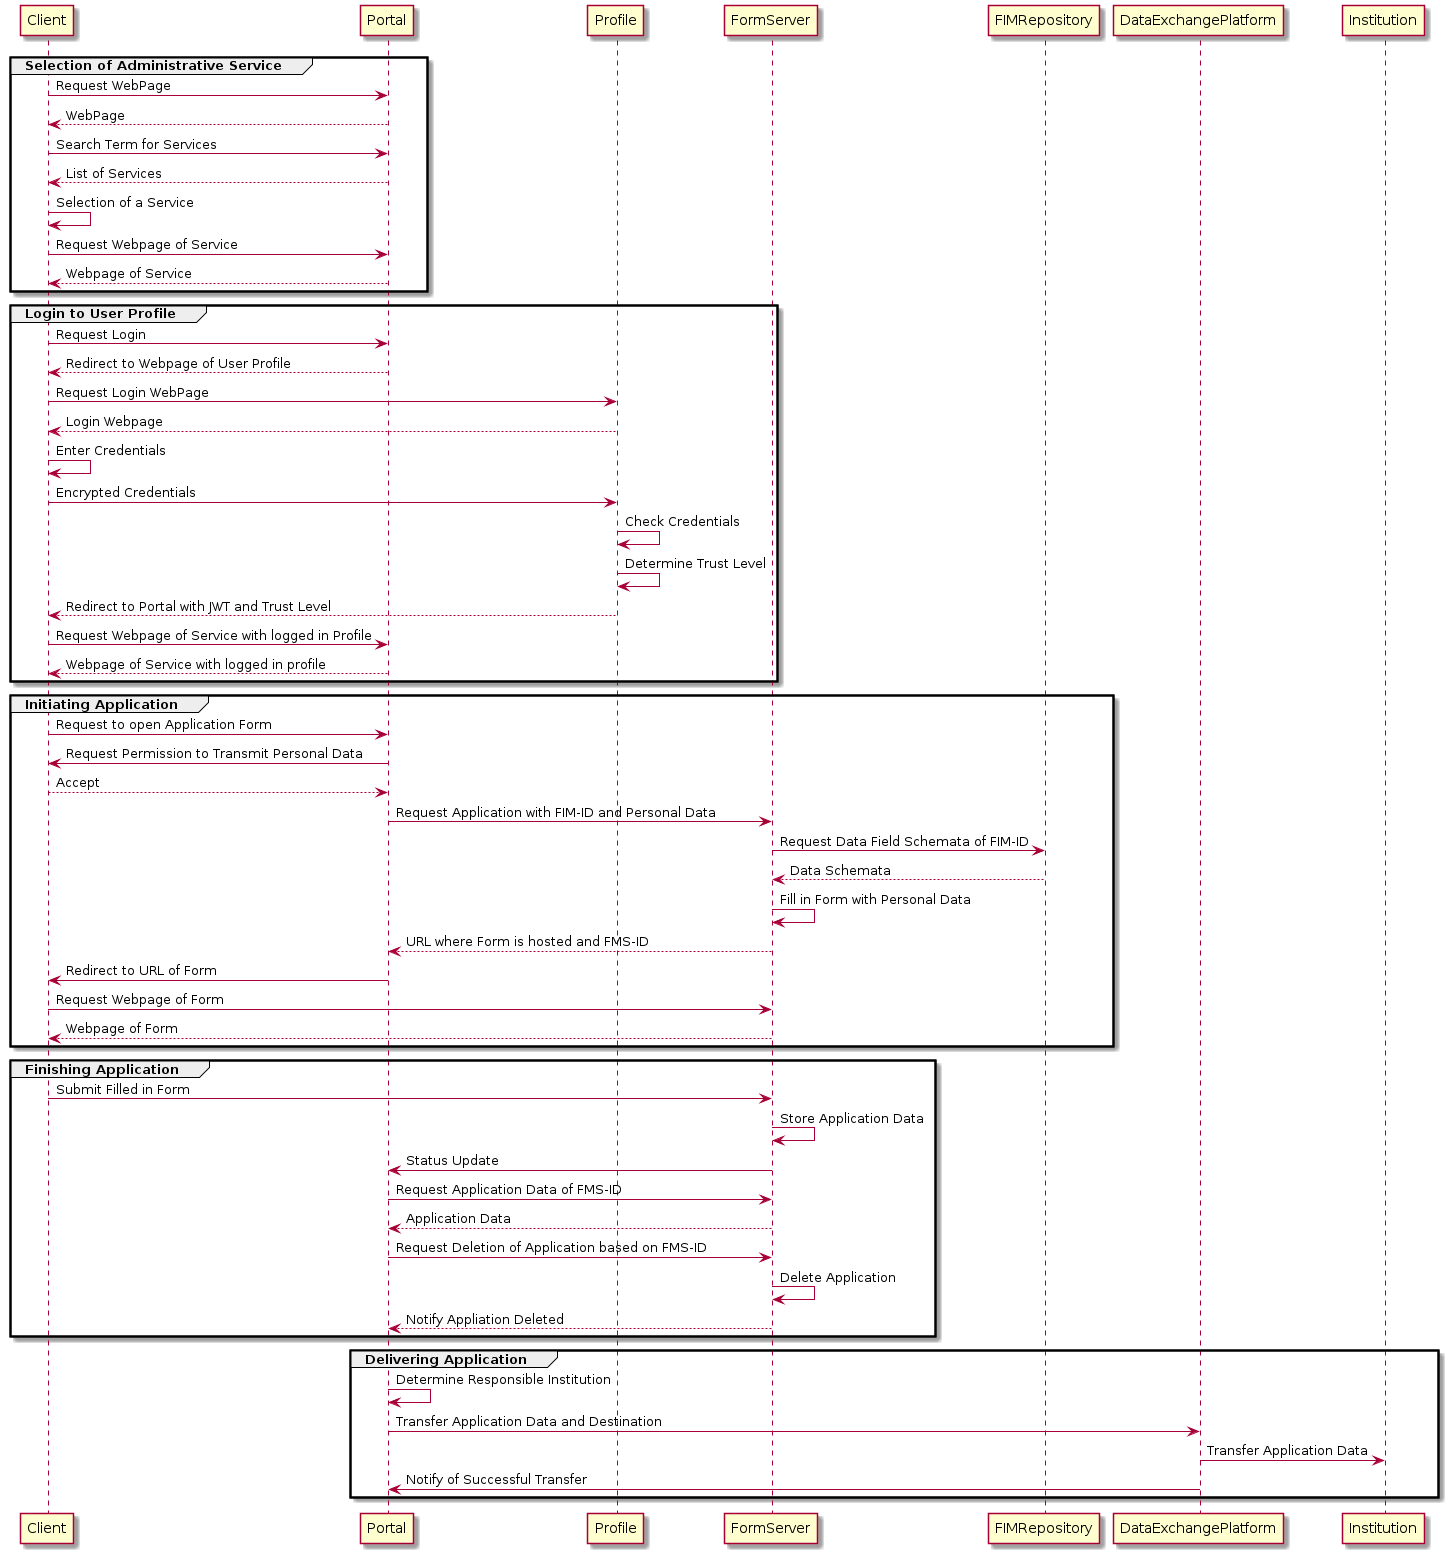
\includegraphics[width=15cm]{Basic Use Case.png}


\chapter{Identity Management}

\section{Functional Requirement Analysis}

\subsection{User Perspective}

\begin{itemize}
    \item The user wants to manage his personal information in one place
    \begin{itemize}
        \item The user wants to CRUD attributes
        \item The user wants SPs to CRUD his attributes
        \item The user wants a user friendly interface where he can CRUD his attributes
        \item In case the user cannot understand an attribute or its possible values, he needs OSS tools which enables him to enter the correct value
        \item The user wants to enter personal information only once (=> SPs should reuse existing attributes)
        \item The user wants a new or modified attributes to be instantly used everywhere
        \item The user wants a deleted attribute to be instantly deleted everywhere
        \item The user wants to have a list of often used attributes, in order to prefill them
    \end{itemize}
    \item The user wants to manage authentication in one place
    \begin{itemize}
        \item The user does not want to authenticate
        \item The user wants that only he has access to the identity
    \end{itemize}
    \item The user wants to manage authorisation in one place
    \begin{itemize}
        \item The user wants to manage who can perform which actions in his name (f.e CRUD attributes, place order, cancel subscription)
        \item The user wants an authorisation to only be granted if he manually approves
        \item The user wants an authorisation to be associated with a single entity, a reason, which actions can be performed and duration of the authorisation
        \item The user wants to communicate with the authorised entity
        \item The user wants to have much information about the authorised entity
        \item The user wants to be able to revoke an authorisation
        \item The user wants to save the history of authorisations
    \end{itemize}
    \item The user wants to use all OSS tools in one place
    \begin{itemize}
        \item Communication through inbox
        \item Subscribe for a service of an SP
        \item Place order in a shop of an SP
        \item ...
    \end{itemize}
    \item The user wants

\end{itemize}

\subsection{Service Provider Perspective}

\begin{itemize}
    \item SPs want to manage personal information of users
    \begin{itemize}
        \item SPs want to CRUD attributes of the user
        \item In case modification of an attribute has strong implications on the operation of a system, the modification of an attribute needs to be limited
        \item SPs want to access personal information already collected by other SPs
        \item SPs want 
    \end{itemize}
    \item identification
    \item authentication
    \item authorisation
    \item 
\end{itemize}

\subsection{OZG Perspective}

\section{IMP Solution Proposal}

\subsection{IMP Functionalities}

The IMP solution aims to replace existing user profiles by enabling users to manage their identity through IMP clients and by integration with service providers.

\subsection{Basic Use Case}

The following diagram describes the concept of how IMP fits within the basic use case of the OZG. It contains some of the previously explained OZG components and an additional component: the IMP client. The IMP client is part of the system architecture and is responsible for identity management. Components related to integration and implementation of IMP are left out in this diagram and are focus of the Integration chapter. 

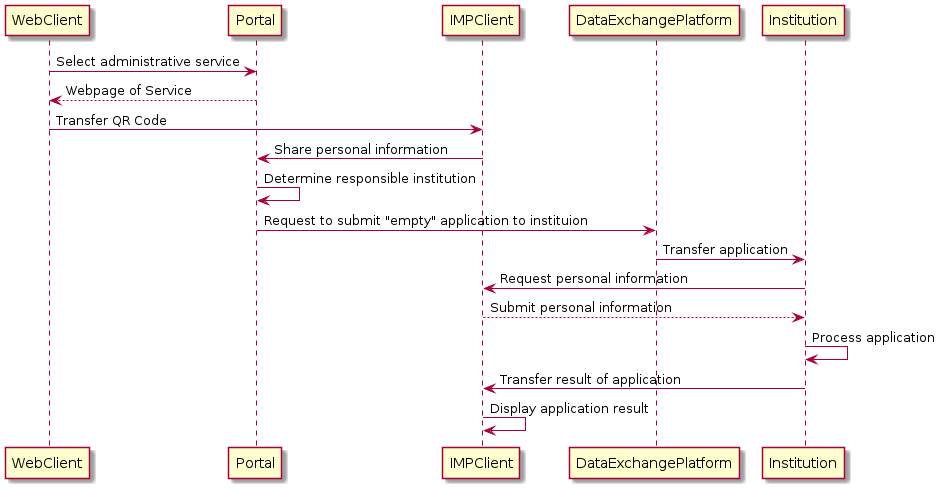
\includegraphics[width=15cm]{Basic Use Case IMP.png}

The selection of an administrative service is online self-service which is not part of identity management an is therefore left to be done through the websites of the administration portal. 

One focus of IMP is to enable the user to be in full control of his identity. It therefore is the goal to execute the basic use case while sharing as little personal information as necessary and sharing personal information only with the components which require it. The main issue of the official execution of the basic use case in this regard is, that the administration portal collects personal information with the purpose of forwarding it to responsible institutions. It is not in the best interest of the user to share all information of an application with the administration portal of a member state when the application is eventually processed by an institution. It would be in the interest of the user to share personal information regarding the application with the institution directly. This way, the user has more differentiated control of which institutions access which personal information. The IMP client in the proposed solution therefore shares personal information directly with the institutions instead of the administration portal.

The result of the application is sent to the IMP client as it contributes to personal information of his identity.

\chapter{IMP Integration Architecture}

\section{Requirement Analysis}

\subsection{Integration Challenges}

The following challenges are a result of the functionalities an IMP system provides in addition to conventional identity management systems. The origin of the challenges is the interoperability of the IMP identity with multiple SPs. It is the purpose of the integration architecture to solve as many of these challenges as possible.

\paragraph{Data Mapping}
If multiple SPs and the user are able to add new attributes, there is the possibility of duplicate attributes with the same meaning but different name. It is also possible for SPs to utilize the same attribute but interpreting its meaning differently.

\paragraph{Identity Attributes}
Service providers are able to add attributes to an identity. It, however, is not clear which information should be added to an IMP system as part of an identity and which information should be stored by the individual SPs. One reason is, that service providers exist for which creation and utilization of personal information is a business model. For those SPs, the secrecy of certain types of personal information is important. One example would be information about product preferences of customers acquired by online retailers for usage with recommender systems.
A guideline could be, to only add attributes to the IMP system, which should be directly managed by users.

\paragraph{Online Self-Service}
SPs might add attributes to the identity of an IMP system which have very special meanings which are not self-explanatory. The attribute might also adhere to a special data format or be conditioned by other attributes of the identity. The modification of the attributes might also require interaction with the system architecture of an SP. In order for the attributes to stay valid, management through online self-service tools which are provided by the system architecture of an SP might be required.

In this case, the self-service tools should be accessible through the IMP systems in a user friendly way.

\paragraph{Attribute Access}
Attributes which were added by a SP might require restrictions towards the user. If for example a subscription status is saved as an attribute, the user should not be able to modify it without permission of the SP.

\subsection{Basic Use Case}

\subsection{Extensions}

\section{Integration Proposal}

\subsection{IMP Connector}

\subsection{Messaging}

\section{Basic Use Case}

\subsection{Sequence Diagrams}

Hier der Anfang einer detaillierteren Beschreibung des Basis Anwendungsfalls basierend auf dem Klassen Diagramm weiter unten.

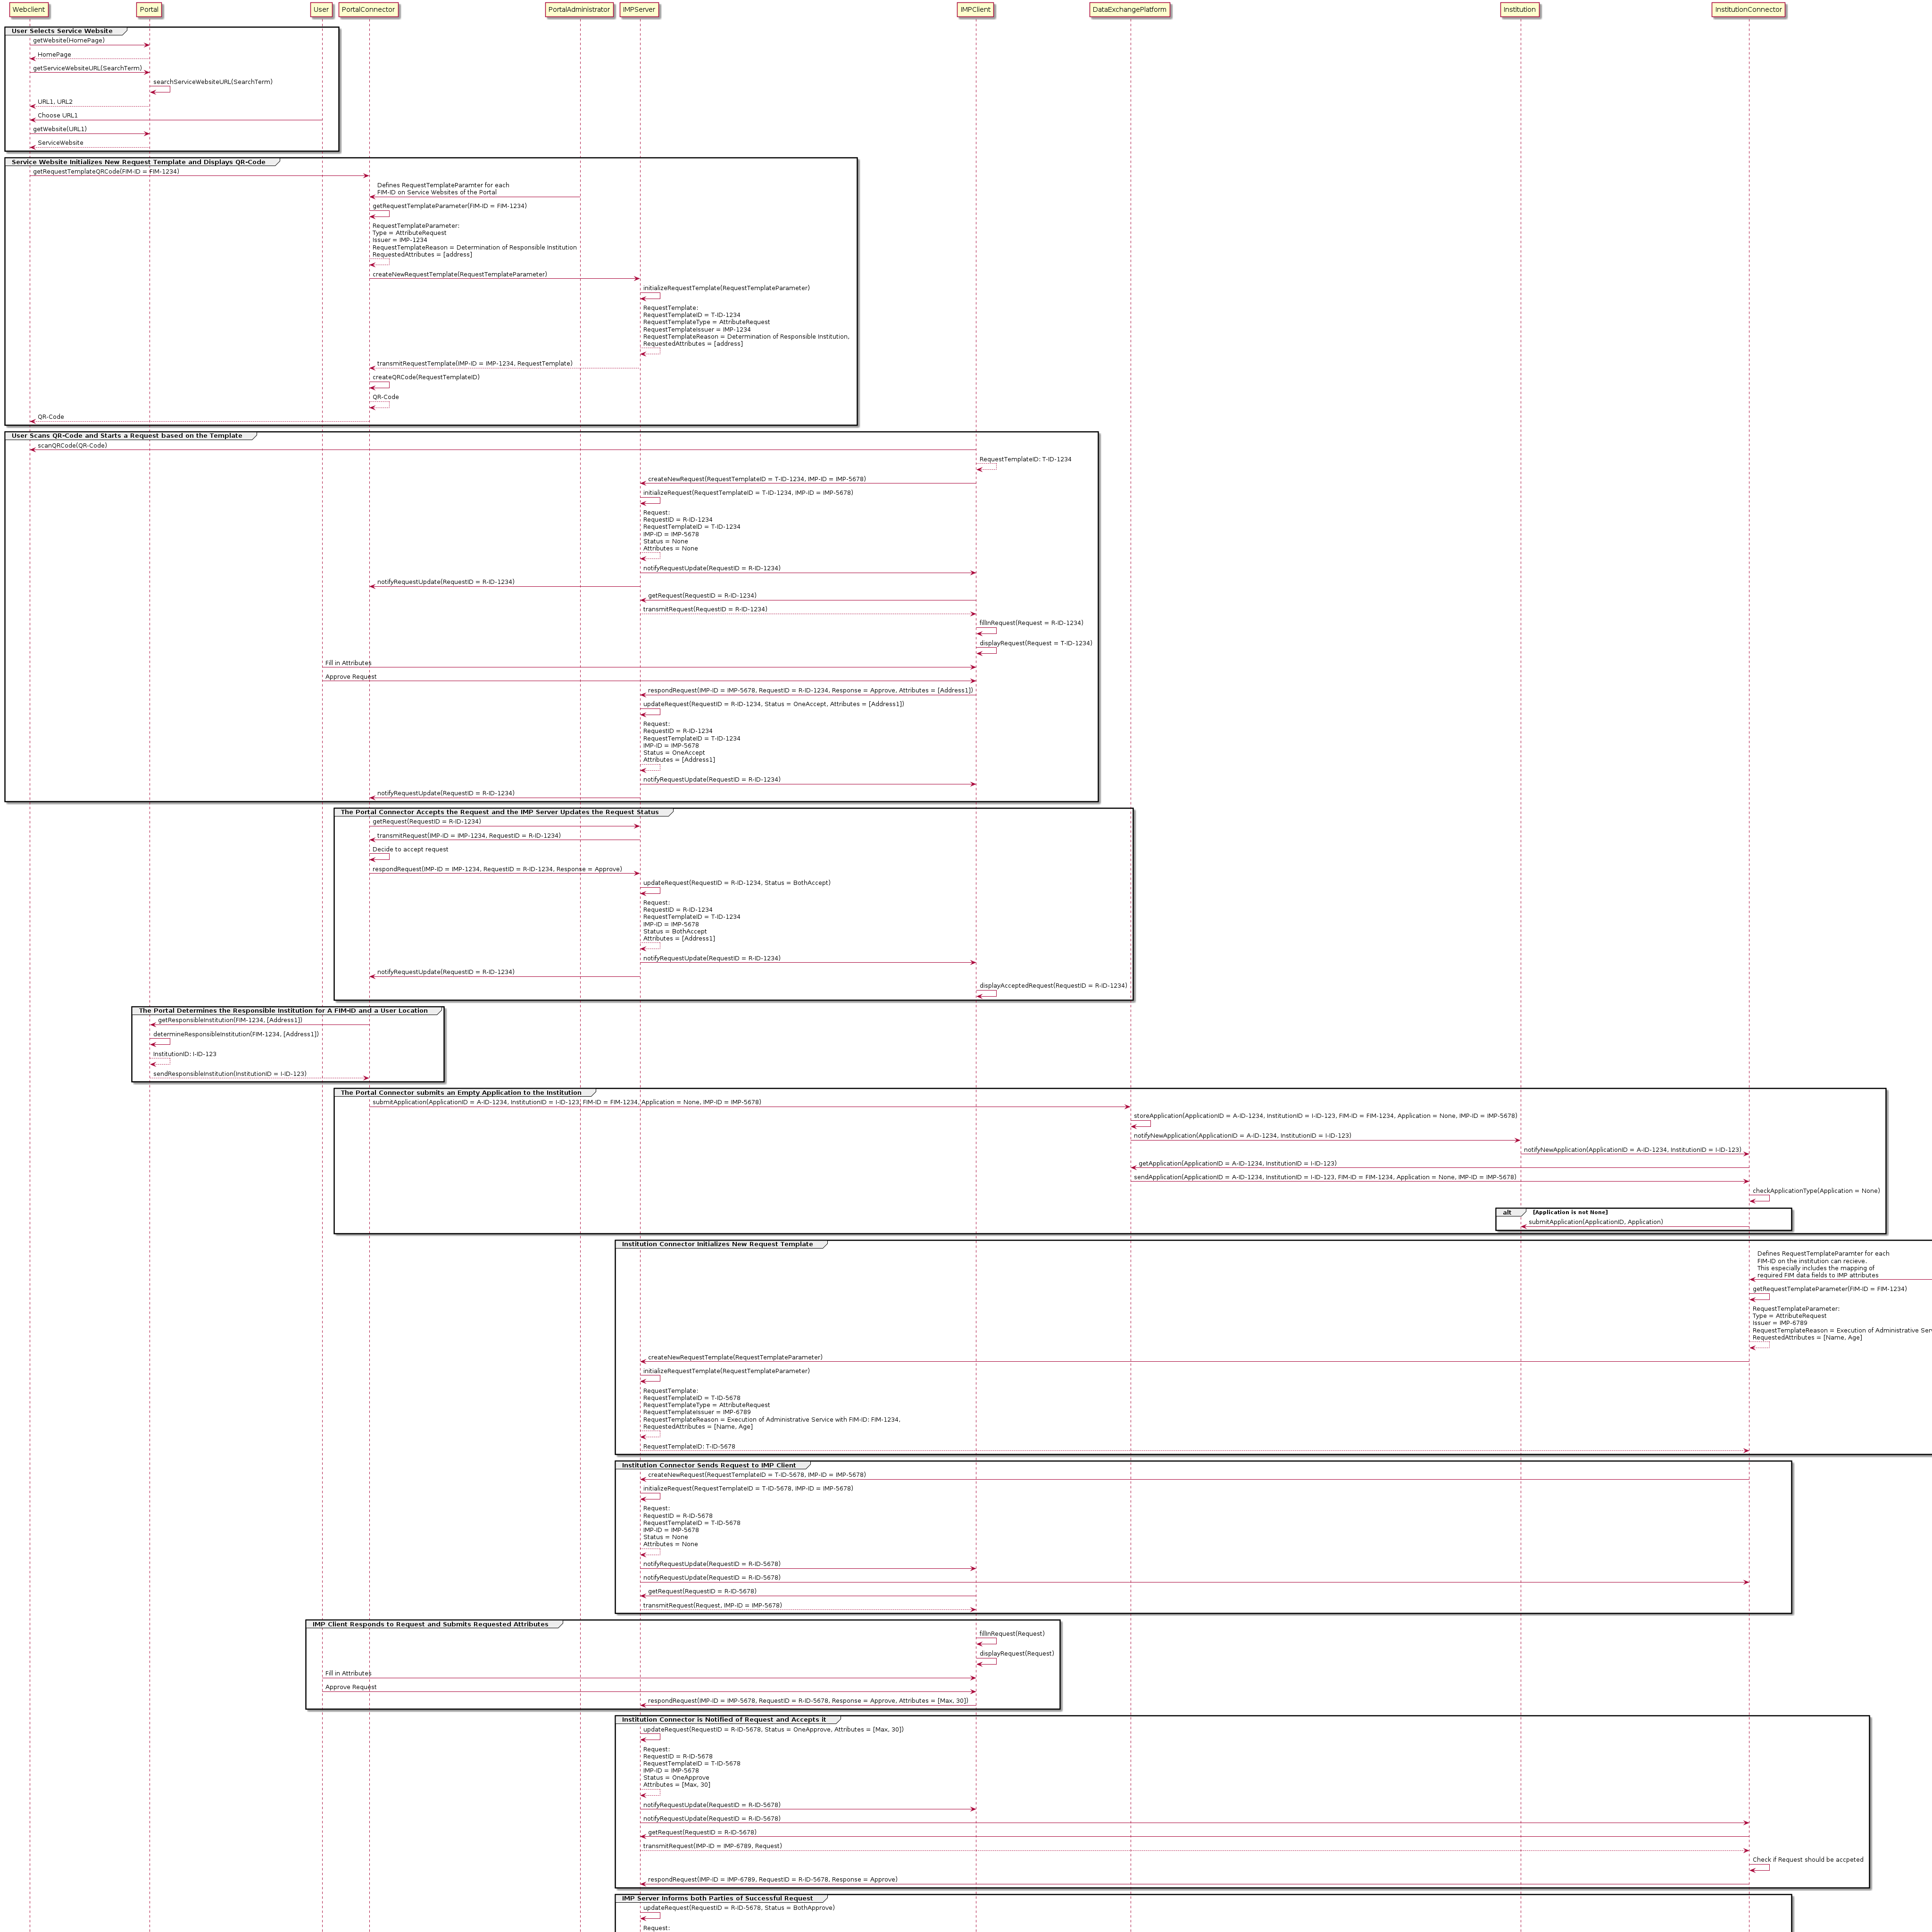
\includegraphics[width=15cm]{Diagrams/out/Sequence Diagram/Sequence Diagram.png}

\subsection{Class Diagram}

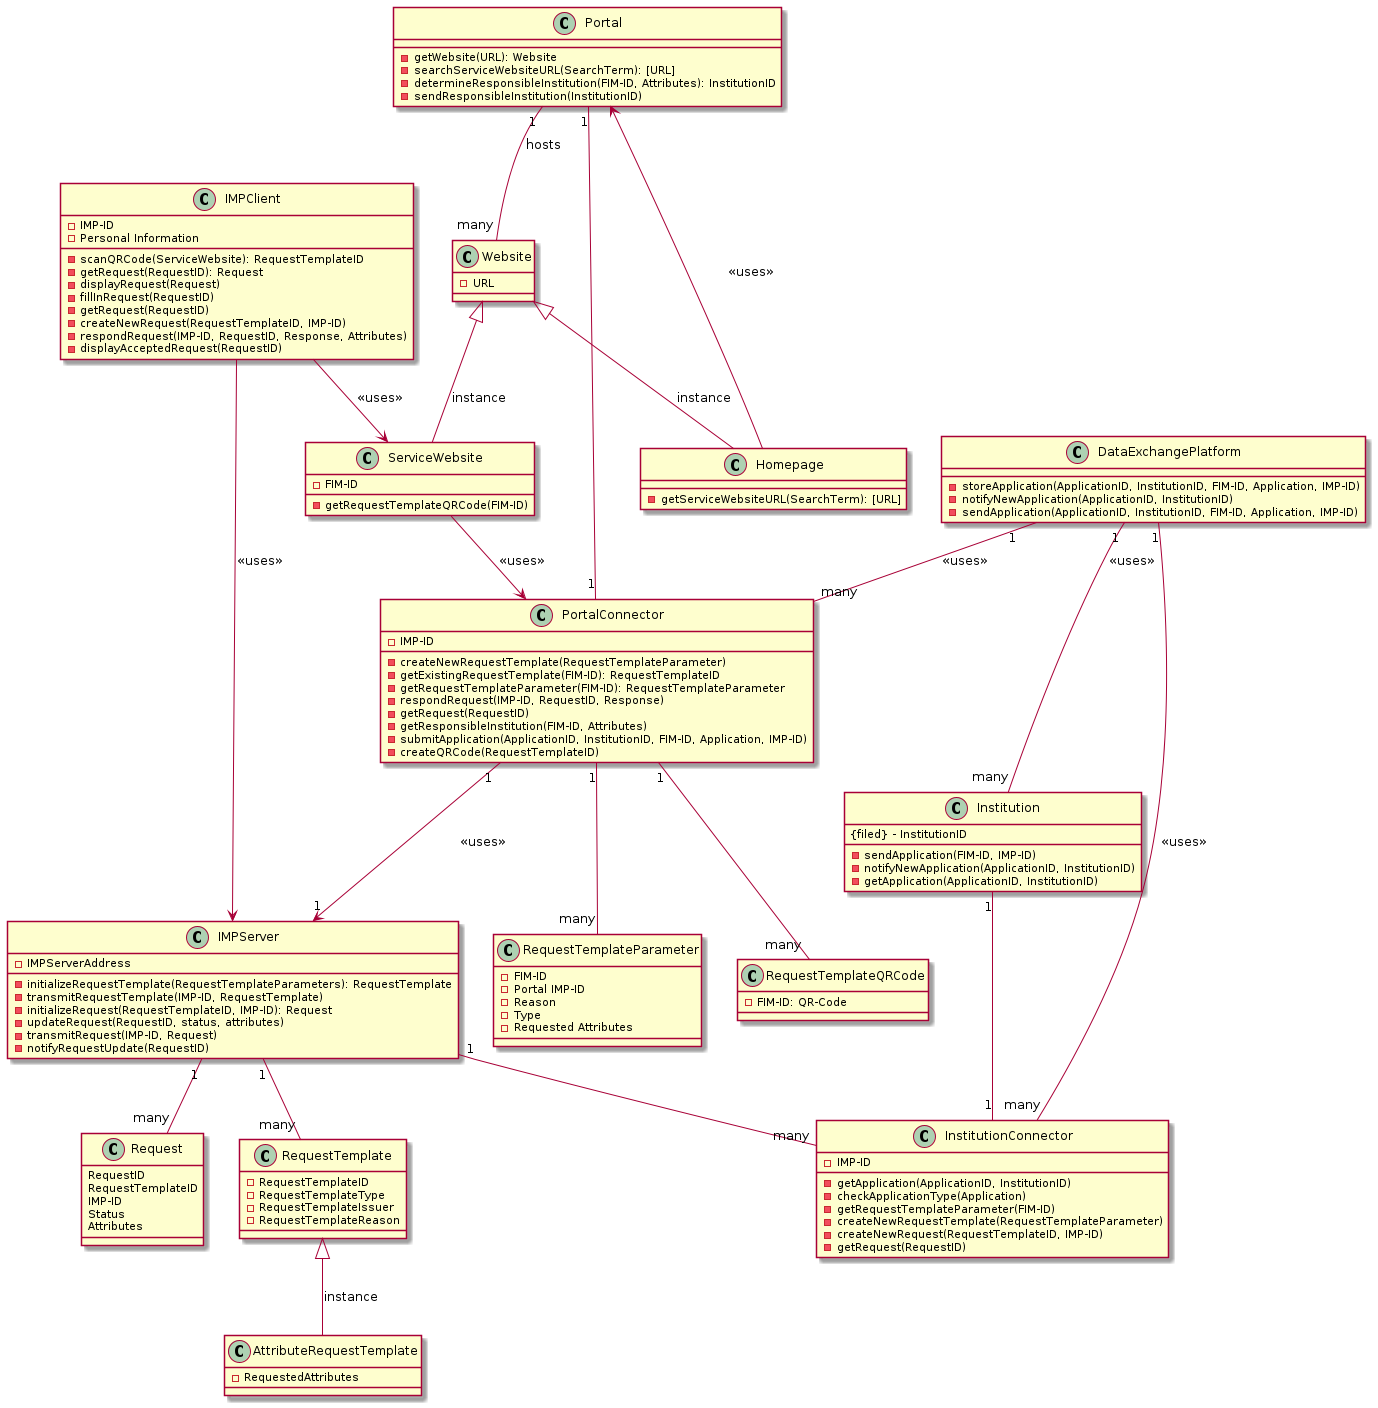
\includegraphics[width=15cm]{Diagrams/out/Class Diagram/Class Diagram.png}

\subsection{Messaging Diagram}

\section{Extension: Inbox}

\section{Extension: Collaboration}

\chapter{Solution Evaluation}

\section{Conclusion}

\chapter{Outlook: Advanced IMP Integration}

\printbibliography


\end{document}
